\documentclass[sigconf]{acmart}

\usepackage{comment, graphicx, algorithm, algorithmic, listings}


\lstdefinelanguage{P4}{
  showlines=true,
  morecomment=[f]{//},
  keepspaces=true,
  basicstyle=\scriptsize\ttfamily,
  emphstyle=\itshape,
  emph={},
  commentstyle=\color{red},
  keywordstyle=\color{blue},
  morekeywords={typedef, header, extern, struct, parser, state, transition, in, out, inout, select, default, control, action, table, apply, if, switch}
}



\AtBeginDocument{%
	\providecommand\BibTeX{{%
			\normalfont B\kern-0.5em{\scshape i\kern-0.25em b}\kern-0.8em\TeX}}}

%% Rights management information.  This information is sent to you
%% when you complete the rights form.  These commands have SAMPLE
%% values in them; it is your responsibility as an author to replace
%% the commands and values with those provided to you when you
%% complete the rights form.
\setcopyright{acmcopyright}
\copyrightyear{2018}
\acmYear{2018}
\acmDOI{10.1145/1122445.1122456}

%% These commands are for a PROCEEDINGS abstract or paper.
%%\acmConference[Woodstock '18]{Woodstock '18: ACM Symposium on Neural
%%  Gaze Detection}{June 03--05, 2018}{Woodstock, NY}
%%\acmBooktitle{Woodstock '18: ACM Symposium on Neural Gaze Detection,
%%  June 03--05, 2018, Woodstock, NY}
%%\acmPrice{15.00}
%%\acmISBN{978-1-4503-XXXX-X/18/06}

\begin{document}
	
	
	\title{TODO}
	
	
	\author{}
	\email{}
	\orcid{}
	\author{}
	\authornotemark[]
	\email{}
	\affiliation{%
		\institution{}
		\streetaddress{}
		\city{}
		\state{}
		\country{}
		\postcode{}
	}
	
	
	\begin{abstract}
		TODO
	\end{abstract}
	
	%%
	%% The code below is generated by the tool at http://dl.acm.org/ccs.cfm.
	%% Please copy and paste the code instead of the example below.
	%% TODO

	
	\keywords{TODO}
	
	
	\maketitle
	
	\section{Introduction}
	% P4 (max 1-1.5 hasáb) - példa (később használandó a többihez) - Máté
	P4~\cite{p4paper} is a high level, domain-specific programming language. It is developed mainly for
describing the data plane layer of packet processing algorithms of different network
devices (e.g. switches, routers) in a protocol and target independent way. Figure~\ref{code:P4} illustrates a P4 program. The program first defines the applied header structure, than the parser part describes how the fields of the defined headers will be set from the input bit stream (input packet). Controller part can modify values of headers' fields and metadatas by applying lookup tables. The dataplane program describes the structure of the tables, the key fields based on that lookups will be executed and the possible results of the lookups, namely the applicable actions. However concrete data of the tables (which actions will be executed with wich parameters for which key values) are defined by the controlplane program, therefore it will not appear in P4. Finally the deparse part defines how the output bitstream (output packet) will be created from the headers.   
	
	
	\section{Related Work}
	% kb 1.5 hasáb
	% felhasznált eszközök  - 
	% egyéb toolok - Vera,  - Gabi
	% Akár gremlin/gráf alapú dolgok, ami nem p4 (akár refactorerl) - mindenki
	

	\section{Motivation}
	% max 1 hasáb - lehet intorba megy - Máté
	% p4-re vannak elemzések kéne fejlesztés segítő eszköz
	% ehhez egységes keretrendszer - vannak már ilyesmik related workben
	


\clearpage

	\section{Analysis framework}


Traditional compilers are designed around passess: the frontend passes parse source code into an intermediate representation (IR), midend passes transforms and adds new information to the IR, and the backend passes create target-specific object code from the IR~\cite{trad-compilers}.  
Modular compilers like P4C improve this design by structuring the passess into a library: backends assemble their own frontends and midends from a catalogue of passes provided by the compiler. Moreover, P4C allows getting information from older states of the IR, as each transformation passes return an immutable IR instance.
Even here, the three-fold separation of frontend-midend-backend have to remain: in order satisfy midend-dependencies, and subsequently, backend-dependencies, the backend must sequentially execute the frontend, the midend, and finally its own passes. 

One goal of the experiment we present here is to relax the three-fold structure and allow passes to reuse (depend on) each other's functionally arbitrarily, and without burdening the compiler programmer with manually finding the right sequence in which to execute these dependencies.

	\subsection{Representation - Architecture} % 4 hasáb - Dániel
	% belső gráf, a koncepció
	% elemzések
	% app megvalósítás

  \begin{figure}
    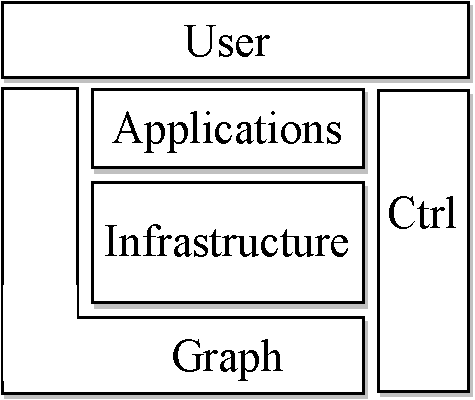
\includegraphics[width=0.18\textwidth]{figures/arch-top.pdf}
    \caption{TODO}\label{fig:arch-top}
  \end{figure}

Besides proposing a more relaxed structure of analysis passes, we had three additional goals in sight: support for different applications through uniform APIs, ease of extensibility, and data-driven programming.

By \textit{supporting different applications} (or backends, in compiler parlance), we mean providing a comfortable way to to implement different end-users services, by reusing the same static code analysis operations.
See Section~\ref{fig:apps} for a few examples of applications built on top of the <NAME>.
In systems with uniform APIs, programmers have to learn only one paradigm to maintain, extend or otherwise alter the system (e.g. in case of P4C, visitors and passes are the main concepts of such a uniform API). 

Figure~\ref{fig:arch-top} depicts how the architecture of <NAME> realizes uniform APIs by relying on a graph database. 
Superficially, applications provide services to the user, by using the services provided by the infrastructurei (see Section~\ref{fig:infra}). In reality, both the infrastructure and applications operate on a large shared graph that collects all our knowledge about the program code. The graph is also exposed to the user to enable custom features (e.g. to attach external loggers, visualizers, and validators). The information in the knowledge graph is accessed using graph queries written in Gremlin (see Section \ref{sec:gremlin}). The impliciation is that each of users, application developers, and infrastructure developers are using one, uniform data structure, and are accessing it using the same mechanism. The seamless collaboration of all these components is managed by the controller component.

  \begin{figure}
    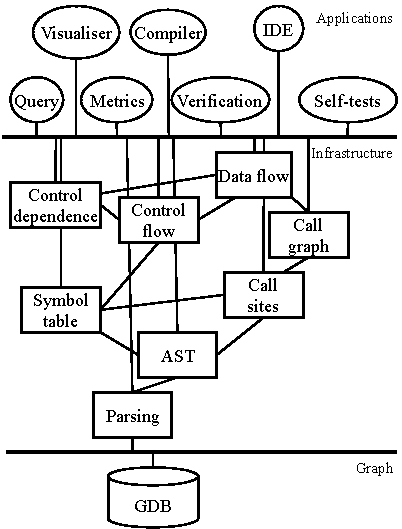
\includegraphics[width=0.3\textwidth]{figures/arch-deps.pdf}
    \caption{TODO}\label{fig:arch-deps}
  \end{figure}

Our second design goal, \textit{ease of extensibility} is illustrated by Figure~\ref{fig:arch-deps}, that elaborates the application and infrastructure layers. 
This arrangement was inspired by declarative build systems and the blackboard pattern used in distributed MI.

The infrastructure consists of a set of interdependent analyser componenents (or passes, in compiler parlance): higher-level analysers can only be executed when lower-level analysers already inserted the necessary knowledge into the graph. To achieve this, analyser components register their needs and provided services to the controller component, and the controller figures out the topological order in which to initiate the analysers. 
Applications provide a user interface (e.g. command line interface) through which their services can be accessed, and similarly to analysers, applications also depend on a subset of the analysers in the infrastructure. But unlike analysers, application are expected to only read (never modify) the graph, and consequently, applications have no dependers. 
In this arrangement, the controller guarantees that when the user executes a work-intensive application, only the minimally necessary components will be performed.
Moreover, when developers introduce new features, this arrangement enables them to think declaratively: instead of thinking about where to insert their feature inside a sequence of operations, they only have to think about their dependencies, i. e. what kind of analysers could help them.

With this, we arrive to our third design goal, \textit{data-driven programming}. Thanks to the uniform graph API and the controller-managed dependecy resolution, programmers are forced to think in terms of data instead of code: they have to look at what code knowledge is in the graph already, figure out what data they want to insert, and possibly find existing analysers that makes writing queries  easier for them. 
The information in the graph is regulated by a well-defined graph schema, and the graph topology is regulated by the well-defined requirements and services of the analysers. Moreover, since the graph instance is detached from the code analysis framework, the programmers can access it by external tools for visualizing, monitoring and validating purposes.
Like this, programmers can almost completely avoid understanding the existing code base, and only have to look at and interact with the data in the graph.  
	
	\subsection{Experts} % 1 hasáb - Dániel
	% kisebb gráf ábra

	\subsection{Testing} % 1 hasáb - Gabi
	There are two main goals with the testing: to test if the analyzes work well; and because it is a quite new tool, it will go through a lot of changes, therefore the possible spoils of the analyses during changes need to be detected. This version of the tool contains unit tests and integration tests to check the functional correctness. 
	
	With the unit tests, our main goal is to check if the analyzes work well. Unit tests need to be fast, therefore they work with the smallest part of the analyses ie. their functions. One function usually define one query of the graph, which insert new edges into it, therefore in these cases, the tests check if the right edges are added to the graph. Using actual P4 source, to test these functions, would be too costly, therefore we define the most simple graphs --, which contains only those edges and vertices, which are necessary for the query -- to check the function.
	
	While unit tests need to be fast, integration tests can be slower, so we can use P4 files as the inputs to test the analyzes. When one analysis needs to be tested, it uses the P4 file, and executes every analysis, that it is based on and the tests will check the result of this running. The tests are predefined, therefore we use a file to store the information of the tested sources and analysis -- which file tests which analyzes with which test classes.
	
	There are two approaches to run these tests. One of them executes all of the defined tests -- i.e. it goes through all of the P4 sources and executes the necessary analyzes and tests the their results -- which is useful to test the whole program and identify regression errors. The other focuses only one analysis and it is useful, when someone actually develop that analysis. This approach run only those tests which are relevant for the analysis.
	
	The architecture gives opportunity to insert the test as an application, which depends on all of the tested analyzes, but these are built into the maven. (TODO - ide még jöhetne talán részletessebben)
	
	% külön modul
	% elvi részei jelenlenek meg
	% ilyen olyan teszt, messziről melyik hogy
	% külön modul
	% elvi részei jelenlenek meg
	% ilyen olyan teszt, messziről melyik hogy
	
	\section{Evaluation}
	
	% scalability measurements  talán 1 hasáb
	% esetleg 1-2 plre hogy futott le - sor alapján? mini mérés
	
	% indítási információk - mindegyiknél /visualisation-nél
	% egyedi elemzések mérése
	\subsection{Visualization} % 0.5 hasáb
	\subsection{Verification} % 1 hasáb - Gabi
	\subsection{Cost analysis} % 1 hasáb - Dániel
	
	\section{Conclusion and Future Work} % 1 hasáb - Máté

\begin{figure*}
\begin{tabular}{|p{3.3cm}|p{5.9cm}|p{7.7cm}|}
\hline
\begin{lstlisting}[language=P4]
// Definitions
typedef bit<9>  egSpec_t;
typedef bit<48> macAddr_t;
typedef bit<32> ip4Addr_t;

// Headers
header ethernet_t {
  macAddr_t dstAddr;
  macAddr_t srcAddr;
  bit<16>   etherType; }
    
header ipv4_t {
  bit<8>    ttl;
  ip4Addr_t srcAddr;
  ip4Addr_t dstAddr;... }
    
struct headers {
  ethernet_t   ethernet;
  ipv4_t       ipv4; }

\end{lstlisting}
&
\begin{lstlisting}[language=P4]
// Parser
parser MyParser(...) {
  state start { transition parse_ethernet; }
  state parse_ethernet {
    packet.extract(hdr.ethernet);
    transition select(hdr.ethernet.etherType) {
      TYPE_IPV4: parse_ipv4;
      default: accept; } }
  state parse_ipv4 {
    packet.extract(hdr.ipv4);
    transition accept; } }
    
// Control    
control MyIngress(...) {
  apply {
    if (hdr.ipv4.isValid()) {
           ipv4_lpm.apply(); }
  }         
  action drop() {
    mark_to_drop(standard_metadata);
  }    
\end{lstlisting}
&
\begin{lstlisting}[language=P4]
  action ipv4_forward(macAddr_t dstAddr, egSpec_t port) {
    standard_metadata.egress_spec = port;
    hdr.ethernet.srcAddr = hdr.ethernet.dstAddr;
    hdr.ethernet.dstAddr = dstAddr;
    hdr.ipv4.ttl = hdr.ipv4.ttl - 1;
  }    
  table ipv4_lpm {
    key = {  hdr.ipv4.dstAddr: lpm;  }
    actions = {
      ipv4_forward;
      drop;
      NoAction;}
    ... }   
}

//Deparser
control MyDeparser(packet_out packet, in headers hdr) {
  apply {
    packet.emit(hdr.ethernet);
    packet.emit(hdr.ipv4);}
}
\end{lstlisting}\\
\hline
\end{tabular}
\caption{P4 example}
  \label{code:P4}
\end{figure*}

\bibliographystyle{ACM-Reference-Format}
\bibliography{tool}

\end{document}
\endinput

